\section{Measurements and evaluation}\label{measurements-and-evaluation}

\subsection{Measurement of relaxation time}\label{relaxation-time}

We measure $T_1$ and $T_2$ once with the spin echo method and $T_2$ again with the Carr-Purcell sequence for each Ga 500 and Ga 600.
\begin{table}[h!]
\centering
\begin{tabular}{c||c|c|c}
probe  &  $T_{1,SE}$ & $T_{2,CP}$ & $T_{2,SE}$ \\
\hline
\hline
Ga 500 & 68.1 & 66.1 & 62.4 \\
\hline
Ga 600 & 99.2 & 84.0 & 78.6 \\
\end{tabular}
\caption{Summary of relaxation time measurements in $ms$}
\label{table1}
\end{table}\\
We can see 3 relations from these measurements: $T_{1} > T_{2}$ and $T_{2,CP} > T_{2,SE}$ for both substances as well as $T_{600} > T_{500}$ for each different method.\\
The first can explained by the interaction between spin and lattice being stronger than the interaction between to spins.\\
The second relation can be explained by looking at the effects of the Carr-Purcell method. This method minimizes the effects of the molecular diffusion and field inhomogeneities, which improves the precision of greater echo times.\\
The third relation can be attributed to the fact that the Ga 500 has higher concentration of hydrogen which leads to lower relaxation time.\\
From $\omega_L = 2\pi\cdot19.8 MHz  $ we can calculate our external field $\vec{B_0}$. And with the characteristic time $\Delta t = 1.29\cdot 10^{-6}s $ for a $90\degree$ pulse we can calculate the solenoidal field $\vec{B_1}$ as well.
\begin{equation}
	B_0 = \dfrac{\omega_L}{\gamma} = 0.48 T
\end{equation}
\begin{equation}
	B_1 = \dfrac{\alpha}{\Delta t \gamma} = 4.3 mT
\end{equation}
with $\gamma$ being the gyromagnetic factor mentioned in section \ref{basics}.\\
\subsection{Chemical shift}\label{chemical-shift}

We measure the peaks and determine which peak is the TMS. After that we calculate the shift with the ppm, which is short for parts per million, given by the .vi and appoint them to a substance from figure \ref{shi2} with the help of the provided reference sheet seen in figure \ref{shi1}. The ppm to calculate the difference was read out of the .vi like in figure \ref{Lab2}. \\
\begin{table}[h!]
\centering
\begin{tabular}{c||c|c|c|c|c}
 & A+ & B+ & C+ & D+ & E+ \\
\hline
\hline
$\Delta$(2nd - TMS) & 2.2 & 2.1 & 2.0 & 3.9 & 2.6 \\
\hline
$\Delta$(3rd - TMS) & 3.9 & 6.9 & 11.6 & 6.3 & 7.5 \\
\hline
$\Delta$(4th - TMS) & 6.3 &  &  &  & \\
\hline
\hline
Substance & fluoroacetone & p-xylol & acetic acid & fluoroacetonitril & toluol \\
\end{tabular}
\caption{Summery of chemical shift in ppm}
\label{table2}
\end{table}\\
Even though the resonance frequency of Flour is a lot higher than the frequency we are using here, we can see the peaks caused by the Flour. They appear because of the spin-spin interaction between Flour and the proton (hydrogen) in FCH$_2$ which lead to 2 different states for the electrons. For both D+ and A+ we can see each of these peaks at 3.9 and 6.3 on both spectra.
\vspace{2mm}\\
From the width of these peaks we can additionally calculate the energy resolution of this measurement as well, as the energy difference between the 2 different states FCH$_2$ can be in, depending on the spin-spin interaction of the electrons.
\begin{equation}\label{E_r}
	\Delta E_{res} = f_{FWHM} \cdot h = 19.9 Hz \cdot 4.136eVs = 8 \cdot 10^{-14}eV
\end{equation}
\begin{equation}\label{E_d}
	\Delta E_{dipole} = f_{\Delta F} \cdot h = 48 Hz \cdot 4.136eVs = 2 \cdot 10^{-13}eV
\end{equation}\\
\subsection{Imaging with NMR}\label{imaging-with-nmr}
\begin{figure}[h]
	\begin{subfigure}{0.32\textwidth}
	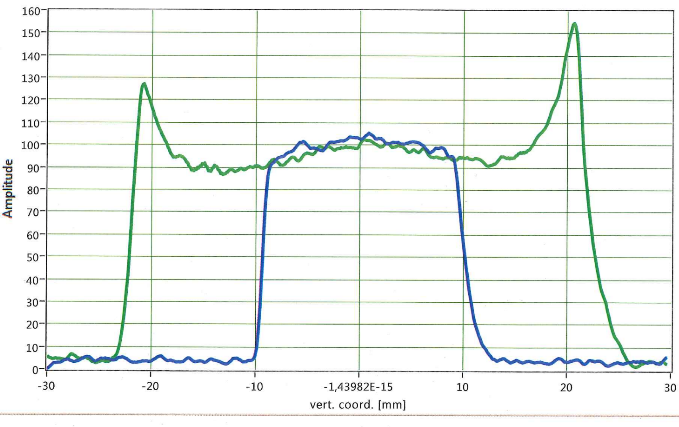
\includegraphics[width=0.9\linewidth ,height=4cm]{images/oil15_50.png}
	\caption{15 mL and 50 mL Oil}
	\label{NMR1}
	\end{subfigure}
	\begin{subfigure}{0.32\textwidth}
	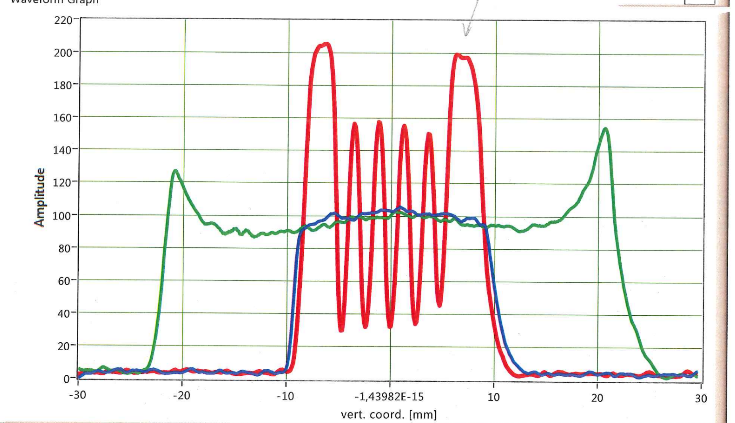
\includegraphics[width=0.9\linewidth ,height=4cm]{images/oil_teflon.png}
	\caption{Oil and Teflon (red graph)}
	\label{NMR2}
	\end{subfigure}
	\begin{subfigure}{0.32\textwidth}
	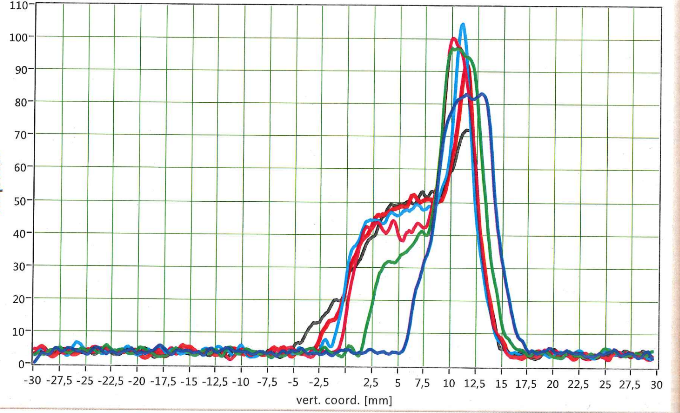
\includegraphics[width=0.9\linewidth, height=4cm]{images/oil_sand.png}
	\caption{Oil on Sand over time}
	\label{NMR3}
	\end{subfigure}
	\caption{NMR imaging 1D}
\end{figure}
First we operate the analyser in the 1D mode. We measure 15 mL oil in a tube and could observe the capillary effect of the liquid on the glass of the tube. Then we filled 50 mL of oil in a tube and observed it. There we could see the boundaries of the analyser. They are caused by the inhomogeneity of the magnetic field if you are too far from the center of the coils. Both of these measurements are seen in figure \ref{NMR1}. \\
The graph the figure \ref{NMR2} is from a tube filled with Teflon and oil, where the low points come from the Teflon layers which aren't NMR-active. \\
We then proceeded to fill an empty tube with 15 mm sand and 4 mm oil on top of it, which we observed in the analyser while the oil was seeping through the sand as shown in figure \ref{NMR3}. While one could think that the seeping of oil into sand could be compared to the diffusion of gas the figure shows it is not the case since it has seemingly random plateaus and drops in the seeping process. \\
For the 2D imaging we inserted various objects into the analyser and looked at the produced image with a LabView .vi. In figure \ref{2DNMR} are some of the images we made.
\begin{figure}[h]
	\begin{subfigure}{0.32\textwidth}
	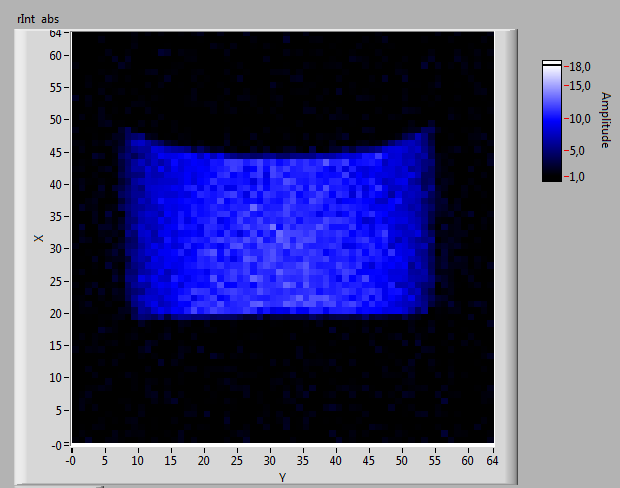
\includegraphics[width=0.9\linewidth ,height=4cm]{2d_image/Oil_Vertical_15_2.png}
	\caption{15 ml Oil 2D}
	\label{2DNMR1}
	\end{subfigure}
	\begin{subfigure}{0.32\textwidth}
	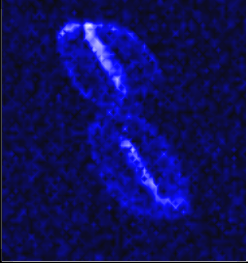
\includegraphics[width=0.9\linewidth ,height=4cm]{2d_image/peanut_5avg_2_3d.png}
	\caption{Peanuts in Shell}
	\label{2DNMR2}
	\end{subfigure}
	\begin{subfigure}{0.32\textwidth}
	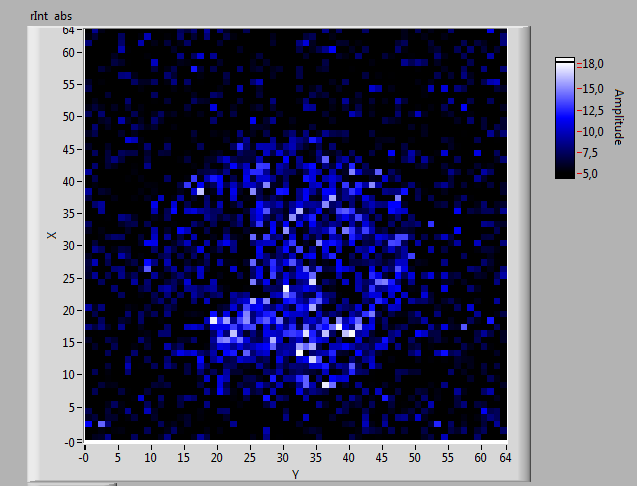
\includegraphics[width=0.9\linewidth, height=4cm]{2d_image/tomato_2.png}
	\caption{A Cherry Tomato}
	\label{2DNMR3}
	\end{subfigure}
	\caption{NMR imaging 2D}
	\label{2DNMR}
\end{figure}
In figure \ref{2DNMR1} you can see the same 15 mL oil tube used for figure \ref{NMR1} but this time imaged in 2D. You can still see the capillary effect at the sides of the tube. \\
In figure \ref{2DNMR2} we imaged a peanut which is still in the shell. The white stripe is the air between the two halves of a single nut. All of this can be observed without ever opening the shell, which illustrates the power of this technique. \\
Finally we took a picture of a tomato slice shown in figure \ref{2DNMR3}. Since a tomato consists of mainly water,  which is not NMR-active, we can't see any kind of shapes on the picture. \\